\chapter{Практическая реализация и экспериментальное исследование нейросетевых методов распознавания различных форм CAPTCHA}

\section{Сравнительный анализ эффективности нейросетевых моделей на текстовых CAPTCHA}

Для распознавания текста с переменной длиной последовательности в задачах CAPTCHA 
наиболее часто применяются следующие из описанных ранее инструменты и архитектуры 
нейронных сетей:

\begin{enumerate}
    \item оптическое распознавание символов (Tesseract OCR);
    \item cверточные рекурентные нейронные сети с функцией потерь Connectionist 
    Temporal Classification (CRNN + CTC);
    \item архитектура последовательного обучения (Sequence-to-Sequence).
\end{enumerate}

С целью выбора наиболее эффективной модели были реализованы и протестированы все 
указанные подходы, после чего была выбрана архитектура, обеспечивающая наилучшую 
точность предсказаний.

Для обучения моделей был сформирован датасет из 100 000 изображений CAPTCHA, 
содержащих случайные последовательности символов длиной от 4 до 7. Такой объем 
данных позволяет добиться высокой обобщающей способности модели и снизить 
вероятность переобучения.

\textbf{Оптическое распознавание символов (OCR Tesseract)}

Изначально была реализована модель с использованием OCR, поскольку такие системы 
изначально разрабатывались для задач оптического распознавания текста. В качестве 
конкретной модели был выбран Tesseract.

Для решения поставленной задачи использовалась предобученная модель Tesseract, 
которая была дообучена на специализированном датасете, содержащем изображения 
CAPTCHA с характерными искажениями. Однако, в ходе экспериментов было установлено, 
что точность распознавания последовательностей символов целиком составляла 0\%, а 
точность для отдельных символов оказалась крайне низкой. Это связано с тем, что 
архитектура Tesseract недостаточно устойчива к искажениям, характерным для 
CAPTCHA, таким как деформация символов, наложение шумов и изменение углов наклона
~\cite{TrainTesseract}.

Таким образом, было принято решение отказаться от использования Tesseract в 
пользу более адаптированных к данной задаче моделей, таких как сверточные 
рекуррентные нейронные сети (CRNN) или модели последовательного обучения 
(Sequence-to-Sequence), обладающие высокой устойчивостью к вариативности и 
искажениям, характерным для CAPTCHA.

\textbf{Рекуррентные сверточные нейронные сети (CRNN)}

Разработанная модель CRNN для распознавания CAPTCHA включает в себя три ключевых 
блока:

\begin{enumerate}
    \item сверточный блок (CNN): предназначен для выделения признаков из 
    изображений CAPTCHA. Включает в себя три последовательных сверточных слоя, а 
    также методы нормализации и уменьшения размерности признакового пространства;
    \item рекуррентный блок (RNN): использует двунаправленные слои GRU, 
    позволяющие модели учитывать зависимость между последовательными символами в 
    CAPTCHA;
    \item выходной слой: полносвязный, который выполняет классификацию каждого 
    символа в последовательности.
\end{enumerate}

В приложении 2 (листинг~\ref{code:crnn}) представлена реализация CRNN-модели на 
языке Python с использованием библиотеки TensorFlow/Keras:

В данной архитектуре применяются слои Dropout для регуляризации, также 
используется l2-регуляризация, BatchNormalization для ускорения обучения и 
повышения устойчивости модели, а также функция softmax для предсказания классов 
символов.

После обучения данной модели результаты оказались превосходящими показатели OCR, 
однако все же не достигли удовлетворительного уровня. В частности, точность 
распознавания всей последовательности символов не превышала 10\%, тогда как 
точность классификации отдельных символов составляла около 70\%.

\textbf{Архитектура последовательного обучения (Sequence-to-Sequence)}

Одним из ключевых элементов реализованной Seq2Seq является механизм внимания, 
который позволяет декодеру динамически фокусироваться на различных частях входной 
последовательности при генерации выходных символов~\cite{seq2seqattention}. Этот 
подход особенно полезен для распознавания CAPTCHA, так как символы в изображениях 
могут иметь разную ориентацию и степень искажения.

Кодировщик, в данной модели принимает входное изображение CAPTCHA и преобразует 
его в компактное представление. Архитектура кодировщика включает:

\begin{enumerate}
    \item четыре сверточных блока, слои пакетной нормализации и слои подвыборки 
    для понижения размерности входных данных;
    \item глобальный усредненный слой для получения векторного представления 
    изображения;
    \item полносвязный слой для финального представления скрытого состояния;
    \item рекуррентный слой для кодирования последовательности, возвращающий 
    последнее скрытое состояние кодировщика.
\end{enumerate}

Декодировщик выполняет пошаговую генерацию выходной последовательности, используя 
скрытое состояние кодировщика. В архитектуру декодировщика входят:

\begin{enumerate}
    \item входной слой для последовательности токенов;
    \item слой вложения, который преобразует входные токены в векторные 
    представления;
    \item рекуррентный слой, обрабатывающий последовательность с учетом скрытого 
    состояния кодировщика;
    \item механизм внимания, который позволяет декодеру учитывать релевантные 
    части входного изображения;
    \item полносвязный слой с функцией активации softmax для предсказания 
    вероятностей символов.
\end{enumerate}

Полная архитектура модели реализована в TensorFlow/Keras и реализация модели 
приведена в приложении 2 (листинг~\ref{code:seq2seq}).

На начальных этапах экспериментов предложенная Seq2Seq-модель показала наилучшие 
результаты среди рассмотренных вариантов. В отличие от OCR- и CRNN-моделей, 
данная архитектура смогла достичь более высокой точности распознавания 
последовательностей символов, что обусловлено применением механизма внимания. 
Дальнейшая работа с моделью была сосредоточена на ее оптимизации и улучшении 
параметров обучения.

\section{Экспериментальные результаты распознавания аудио- и графических CAPTCHA}

\textbf{CAPTCHA в графическом формате}

CAPTCHA в формате изображений, на сегодняшний день, широко используется для 
защиты ресурсов от автоматизированных ботов и может быть реализована несколькими 
способами. Как правило, такие CAPTCHA направлены на проверку способности 
пользователя распознавать и интерпретировать объекты на изображении. Наиболее 
распространены два варианта реализации (оба варианта реализации проиллюстрированы 
на рис.~\ref{fig:example}):

\begin{enumerate}
    \item цельное изображение, содержащее несколько объектов, частично размытых 
    или искаженных, при этом изображение разбито на сетку 3×3 или 4×4. 
    Пользователю предлагается выбрать ячейки, содержащие объекты определенного 
    класса (например, автобусы или светофоры);
    \item составное изображение, сформированное из 9 или 12 отдельных фрагментов 
    (изображений), каждый из которых представляет собой независимое изображение 
    -- зачастую низкого качества, с наложением артефактов или шумов. Задача 
    пользователя -- выбрать те изображения, где присутствует нужный объект.
\end{enumerate}

\begin{figure}[H]
    \begin{minipage}[h]{0.49\linewidth}
        \center{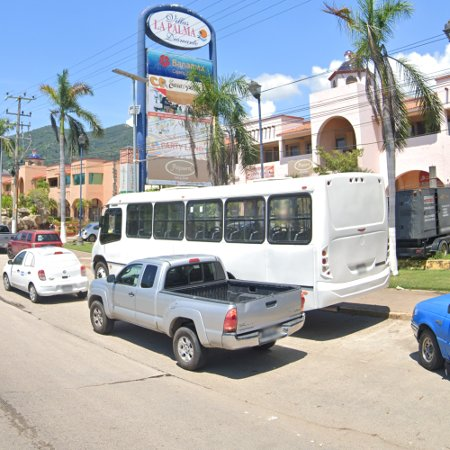
\includegraphics[width=1\linewidth]{imgs/imagecaptcha/6.jpg} \\ 
        а)}
    \end{minipage}
    \hfill
    \begin{minipage}[h]{0.49\linewidth}
        \center{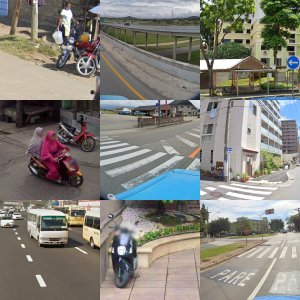
\includegraphics[width=1\linewidth]{imgs/imagecaptcha/8.jpg} \\ 
        б)}
    \end{minipage}
    \caption{Изображения графических CAPTCHA с размером сетки 3×3: а) -- цельное, 
    б) -- составное.}
    \label{fig:example}
\end{figure}
\vspace{-0.85cm}

Такие CAPTCHA требуют от системы автоматического анализа способности как к 
глобальному восприятию изображения, так и к локальной интерпретации его 
фрагментов. Соответственно, модель, предназначенная для решения данной задачи, 
должна поддерживать:

\begin{enumerate}
    \item классификацию объектов на уровне отдельных изображений (для CAPTCHA, 
    основанных на отдельных картинках в сетке);
    \item локализацию и сегментацию объектов с высокой точностью, чтобы 
    корректно определить границы объектов в пределах ячеек, особенно в случаях, 
    когда объект может частично заходить за границу между ячейками.
\end{enumerate}

Для решения этих задач были рассмотрены следующие современные архитектуры 
нейронных сетей, которые были рассмотрены ранее:

\begin{enumerate}
    \item YOLO (You Only Look Once) -- однопроходная модель, объединяющая 
    классификацию и регрессию ограничивающих рамок в одной сверточной 
    архитектуре; отличается высокой скоростью и хорошей точностью~\cite{yolo};
    \item Faster R-CNN -- двухступенчатая модель, в которой сначала генерируются 
    области предложений, а затем выполняется классификация и уточнение рамок; 
    обладает высокой точностью, но уступает в скорости~\cite{fasterrcnn};
    \item DETR (DEtection TRansformer) -- основана на архитектуре трансформеров, 
    что позволяет эффективно моделировать глобальные взаимосвязи между объектами. 
    Подходит для задач с большим количеством контекстных зависимостей, но требует 
    больше ресурсов для обучения~\cite{detr}.
\end{enumerate}

Среди этих архитектур было принято решение использовать YOLOv8 по следующим 
причинам~\cite{UltralyticsYOLOv8}:

\begin{enumerate}
    \item высокая производительность: YOLOv8 показывает высокую скорость 
    обработки изображений без значительного ущерба для точности, что критично в 
    условиях, когда необходимо обрабатывать CAPTCHA в реальном времени;
    \item гибкость и масштабируемость: модель предоставляет множество 
    предобученных вариантов с различной глубиной и числом параметров (версии n, 
    s, m, l, x), что позволяет использовать как на слабых, так и на 
    производительных устройствах;
    \item широкая поддержка и документация: YOLOv8 имеет активное сообщество, 
    подробную документацию и регулярно обновляется, что значительно упрощает 
    интеграцию и адаптацию модели под пользовательские задачи;
    \item поддержка сегментации: в отличие от более ранних версий, YOLOv8 
    поддерживает не только детекцию, но и сегментацию объектов, что особенно 
    важно для задач, где необходимо точно определить область объекта внутри 
    изображения;
    \item дообучение на пользовательских данных: YOLOv8 позволяет эффективно 
    дообучать модель на собственных датасетах, что особенно важно при работе с 
    CAPTCHA-изображениями, содержащими специфические классы объектов и 
    нестандартные искажения.
\end{enumerate}

Кроме того, модель YOLOv8 была успешно протестирована в задачах, близких по 
структуре к CAPTCHA: детекции дорожных знаков, транспортных средств, пешеходов и 
других объектов в сложных условиях съемки, что подтверждает ее универсальность и 
применимость к рассматриваемой задаче.

Таким образом, YOLOv8 является наиболее сбалансированным выбором, обеспечивающим 
как точную классификацию, так и локализацию объектов в условиях ограниченных 
ресурсов и с возможностью адаптации под специфику визуальных CAPTCHA.

В качестве основной архитектуры была выбрана модель YOLOv8m-seg, поддерживающая 
сегментацию объектов. Она представляет собой сбалансированное решение между 
качеством распознавания, производительностью и требованиями к аппаратному 
обеспечению. Благодаря своей универсальности, модель подходит как для задач 
классификации, так и для задач детектирования и сегментации, что особенно важно 
при работе с CAPTCHA, содержащими зашумленные или плохо различимые объекты.

Преимущества YOLOv8m-seg заключаются в следующем:

\begin{enumerate}
    \item наличие встроенной поддержки сегментации объектов, что особенно важно 
    при необходимости выделения фрагментов изображений;
    \item возможность использования предобученных весов, сокращающих время на 
    обучение и повышающих стартовую точность;
    \item высокая скорость инференса по сравнению с другими моделями сегментации 
    (например, Mask R-CNN или DETR);
    \item встроенные средства аугментации (изменения яркости, повороты, 
    масштабирование и пр.);
    \item удобный интерфейс через библиотеку ultralytics, позволяющий быстро 
    запускать обучение, логировать метрики и визуализировать результаты;
    \item полная совместимость с аннотациями в формате YOLO, полученными из CVAT.
\end{enumerate}

Перед запуском обучения структура данных была организована в соответствии с 
требованиями YOLOv8: директории train и val содержали соответствующие изображения 
и файлы разметки, а в .yaml файле конфигурации были указаны пути к выборкам и 
список классов.

Обучение проводилось на 35 эпохах при размере изображений 640×640 пикселей и 
размере батча 8. Использование предобученных весов позволило достичь стабильного 
снижения функции потерь с первых эпох, а встроенные механизмы аугментации 
способствовали улучшению обобщающей способности модели. Программный код для 
обучения модели представлен в приложении 3 (листинг~\ref{code:recognize}).

\textbf{CAPTCHA в аудио формате}

Аудио CAPTCHA представляет собой элемент веб-страницы, содержащий ссылку на 
звуковой фрагмент, включающий наложенные шумы и голосовую запись. Основной целью 
таких заданий является затруднение автоматического распознавания, однако с 
использованием современных технологий распознавания речи возможно достичь высокой 
точности при автоматической обработке подобных аудиозаписей.

В настоящей работе для решения задачи автоматического распознавания аудио CAPTCHA 
был использован облачный сервис Google Web Speech API. Данный API предоставляет 
широкий спектр возможностей, делающих его эффективным инструментом для 
автоматического распознавания речи. Среди ключевых преимуществ API можо выделить 
следующие:

\begin{enumerate}
    \item высокая точность распознавания -- алгоритмы Google обучены на обширных 
    корпусах данных и демонстрируют высокую устойчивость к шумам, что особенно 
    важно при обработке аудиофайлов CAPTCHA, содержащих искажения;
    \item многоязычная поддержка -- API поддерживает большое количество языков и 
    диалектов, обеспечивая гибкость при использовании в различных регионах;
    \item облачная инфраструктура -- использование облачных вычислений позволяет 
    обрабатывать аудиофайлы быстро и без необходимости локального развёртывания 
    сложных моделей;
    \item поддержка различных форматов -- API может работать с аудиофайлами в 
    форматах, пригодных для высококачественного распознавания речи;
    \item удобство интеграции -- API предоставляет хорошо документированный 
    интерфейс, который позволяет быстро встроить функциональность распознавания 
    речи в существующие системы.
\end{enumerate}

Процесс автоматической обработки аудиофайла, полученного с web-страницы, можно 
условно разделить на три основных этапа:

\begin{enumerate}
    \item преобразование формата аудиофайла: исходный файл, как правило, 
    представлен в формате MP3, который использует сжатие с потерями и не подходит 
    для качественного распознавания, поэтому для обеспечения совместимости с 
    сервисом распознавания, аудиофайл перекодируется в формат WAV, отличающийся 
    меньшим уровнем искажения сигнала; для этой цели применяется мультимедийный 
    инструмент с открытым исходным кодом -- ffmpeg, который обеспечивает высокую 
    гибкость при работе с аудиоданными~\cite{ffmpeg};
    \item распознавание речи: на этом этапе перекодированный файл передаётся в 
    облачный сервис Google Web Speech API, где происходит извлечение текстовой 
    информации из аудиопотока;
    \item сохранение результата: полученный в результате распознавания текст 
    сохраняется для дальнейшего использования, в частности, для автоматического 
    ввода в текстовое поле формы на веб-странице.
\end{enumerate}

Таким образом, применение облачного сервиса Google позволяет эффективно решать 
задачу автоматического распознавания CAPTCHA в аудиоформате, демонстрируя высокую 
точность при обработке и устойчивость к шумам, характерным для подобных заданий.

Описанный алгоритм можно представить в виде следующей блок-схемы (рис.~
\ref{fig:recognize-audio}). Программная реализация алгоритма тестирования 
представлена в приложении 1 (листинг~\ref{code:audiocaptcha}).

\begin{figure}[H]
    \centering
    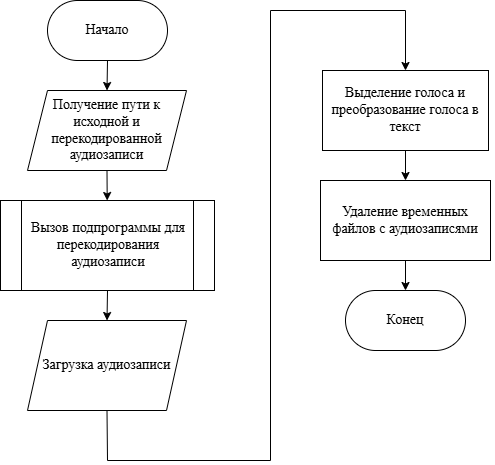
\includegraphics[width=0.6\linewidth]{
        imgs/audiocaptcha/recognize_audiocaptcha.png
    }
    \caption{Блок-схема процесса распознавания Audio CAPTCHA.}
    \label{fig:recognize-audio}
\end{figure}
\vspace{-0.85cm}

\section{Разработка и исследовательский вклад в автоматизацию решения CAPTCHA}

\textbf{Тестирование Sequence-to-Sequence модели для текстовых CAPTCHA}

Как было установлено в предыдущих разделах, модель последовательного 
преобразования (Seq2Seq) продемонстрировала наилучшие результаты среди 
рассмотренных архитектур. Следующим этапом работы являлась оптимизация параметров 
модели, включая веса и коэффициенты регуляризации, с целью ускорения сходимости, 
минимизации риска переобучения и повышения точности распознавания целевых 
последовательностей.

Для проведения экспериментов исходный набор данных, содержащий 100 000 
изображений, был случайным образом перемешан и разделен на три подмножества: 
обучающее, тестовое и валидационное в соотношении 80:10:10. Обучающая выборка 
использовалась непосредственно для обучения модели, валидационная -- для контроля 
качества процесса обучения на каждой эпохе, а тестовая -- для окончательной 
оценки модели на данных, с которыми она ранее не сталкивалась. В качестве 
основных метрик качества модели использовались функция потерь (loss) и точность 
(accuracy), рассчитываемая для каждого символа последовательности.

В процессе многократного обучения были экспериментально определены оптимальное 
количество эпох и значения гиперпараметров, обеспечивающие эффективное снижение 
функции потерь до приемлемых значений. График сходимости функции потерь 
представлен на рис.~\ref{fig:loss}.

\begin{figure}[H]
    \centering
    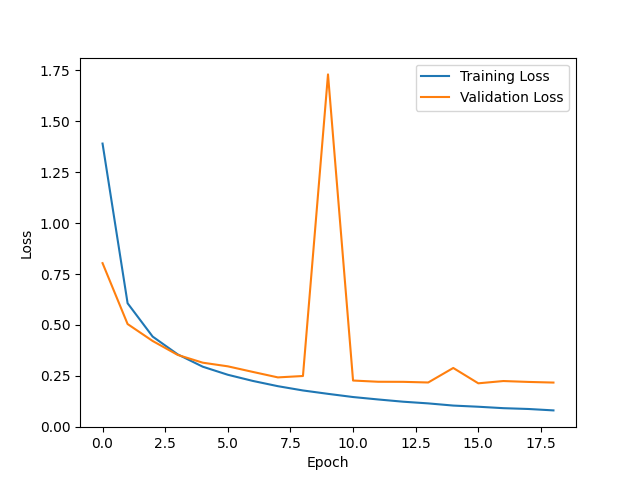
\includegraphics[width=0.8\linewidth]{imgs/textcaptcha/Model_loss.png}
    \caption{График изменения значений функции потерь в процессе обучения модели 
    для решения текстовых CAPTCHA.}
    \label{fig:loss}
\end{figure}
\vspace{-0.85cm}

Для предотвращения переобучения использовался механизм ранней остановки, согласно 
которому обучение прекращалось при отсутствии уменьшения значения функции потерь 
на валидационной выборке в течение трех последовательных эпох. В данном 
эксперименте обучение завершилось на 18-й эпохе. На графике видно, что функция 
потерь стабилизировалась после 10 эпохе, поэтому 10 эпоха является балансом между 
точностью распознавания последовательностей и скоростью обучения модели.

Анализ графика сходимости функции потерь показывает наличие резкого увеличения ее 
значения на 9-й эпохе, что может быть обусловлено следующими факторами:
\begin{enumerate}
    \item перемешивание данных перед каждой эпохой могло привести к образованию 
    несбалансированной выборки, содержащей значительное число сложных примеров.
    \item динамическое изменение скорости обучения, осуществляемое с помощью 
    механизма регулирования скорости обучения (learning rate scheduler), могло 
    повлиять на изменение функции потерь.
\end{enumerate}

Окончательная точность распознавания отдельных символов составила 0.9263.

После подбора оптимальных значений гиперпараметров модель была сохранена и 
протестирована на тестовой выборке. Точность распознавания последовательностей 
различной длины представлена в таблице~\ref{tab:probability}.

\begin{table}[H]
    \centering
    \caption{Точность предсказаний для последовательностей различной длины.}
    \begin{tabular}{|l|l|}
        \hline
        Длина последовательности & Точность распознавания \\
        \hline
        4 символа & 0.9305 \\
        \hline
        5 символов & 0.7450 \\
        \hline
        6 символов & 0.4575 \\
        \hline
        7 символов & 0.1915 \\
        \hline
    \end{tabular}
    \label{tab:probability}
\end{table}

Также была построена матрица ошибок, позволяющая проанализировать частоту и 
характер ошибок модели при классификации различных классов. Данная матрица 
приведена на рис.~\ref{fig:cm}. Программная реализация для тестирования моедли 
представлена в приложении 2 (листинг~\ref{code:test-model}).

\begin{figure}[H]
    \centering
    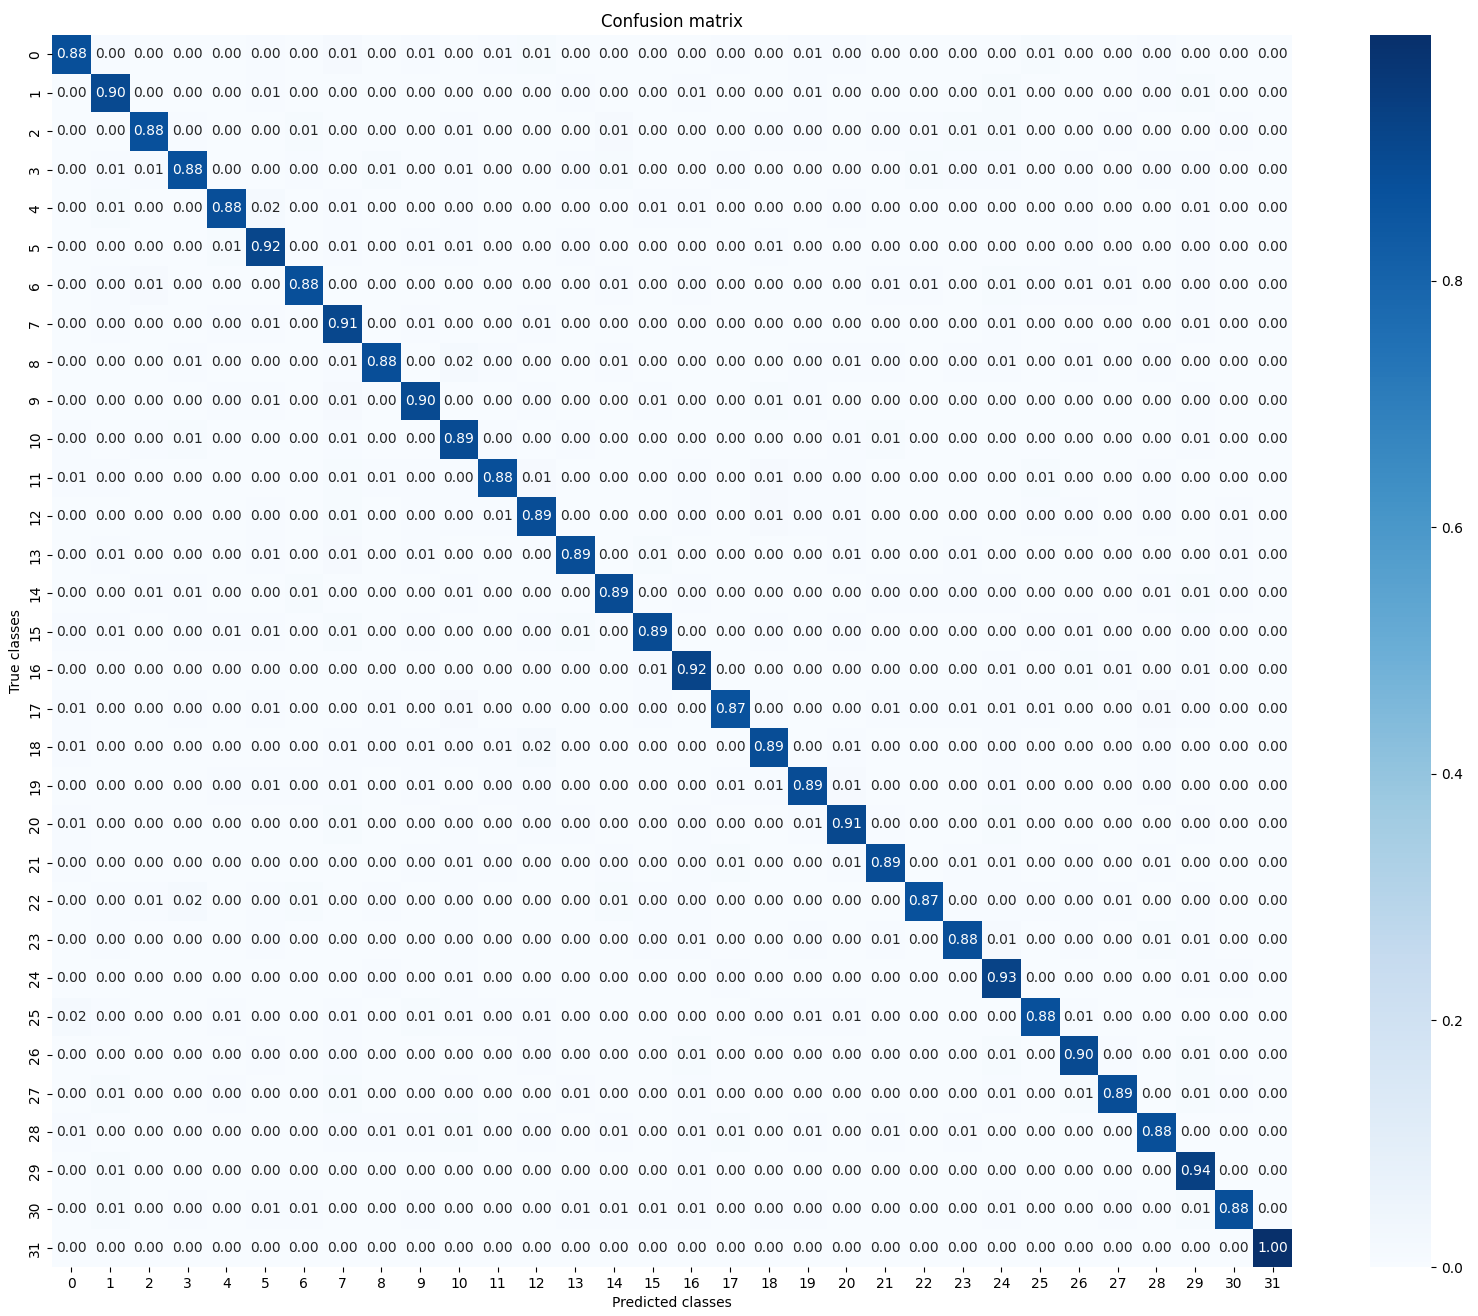
\includegraphics[width=1\linewidth]{imgs/textcaptcha/Confusion_matrix.png}
    \caption{Матрица ошибок для обученной модели для решения текстовых CAPTCHA.}
    \label{fig:cm}
\end{figure}
\vspace{-0.85cm}

Анализ полученных результатов показывает, что точность распознавания 
последовательностей значительной длины остается относительно низкой. Это можно 
объяснить высокой зависимостью модели Seq2Seq от объема обучающих данных: для 
эффективного обобщения признаков, извлекаемых из изображений, требуется 
значительное количество примеров. Следовательно, увеличение размера обучающего 
набора данных потенциально может способствовать повышению точности модели, 
однако это также накладывает дополнительные требования к вычислительным ресурсам, 
необходимым для ее обучения.

\textbf{Тестирование модели YOLOv8 для графических CAPTCHA}

Результаты обучения модели на основе YOLO отслеживались по ключевым метрикам 
(IoU, Precision, Recall, Loss), которые визуализировались автоматически. Примеры 
графиков с результатами обучения приведены ниже:

\begin{figure}[H]
    \centering
    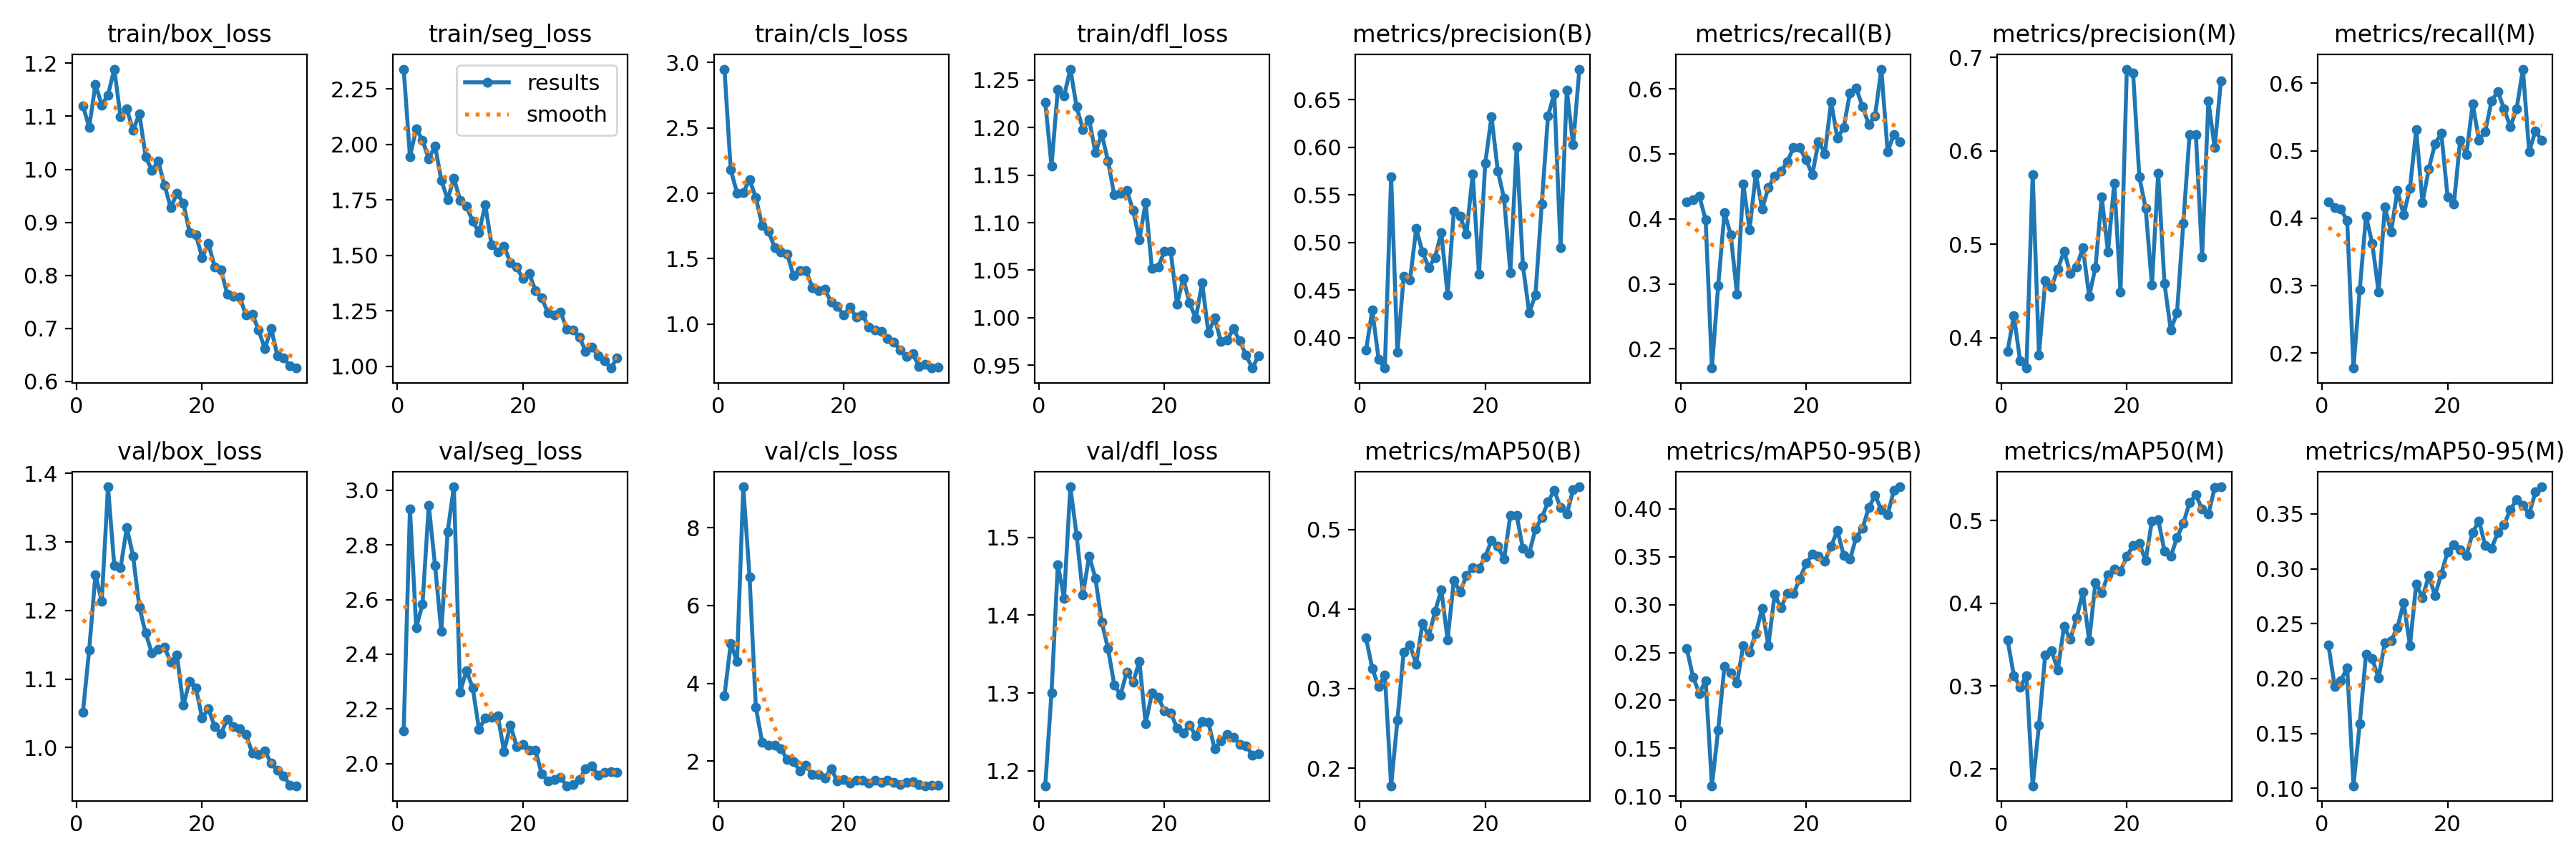
\includegraphics[width=1\linewidth]{imgs/imagecaptcha/results.png}
    \caption{Изменение ключевых метрик в процессе обучения модели YOLOv8.}
    \label{fig:metrics}
\end{figure}
\vspace{-0.85cm}

Также, была построена нормализованная матрица ошибок для определения точности 
предсказания необходимых классов на валидационной выборке, которая представлена 
на рис.~\ref{fig:confusion}.

\begin{figure}[H]
    \centering
    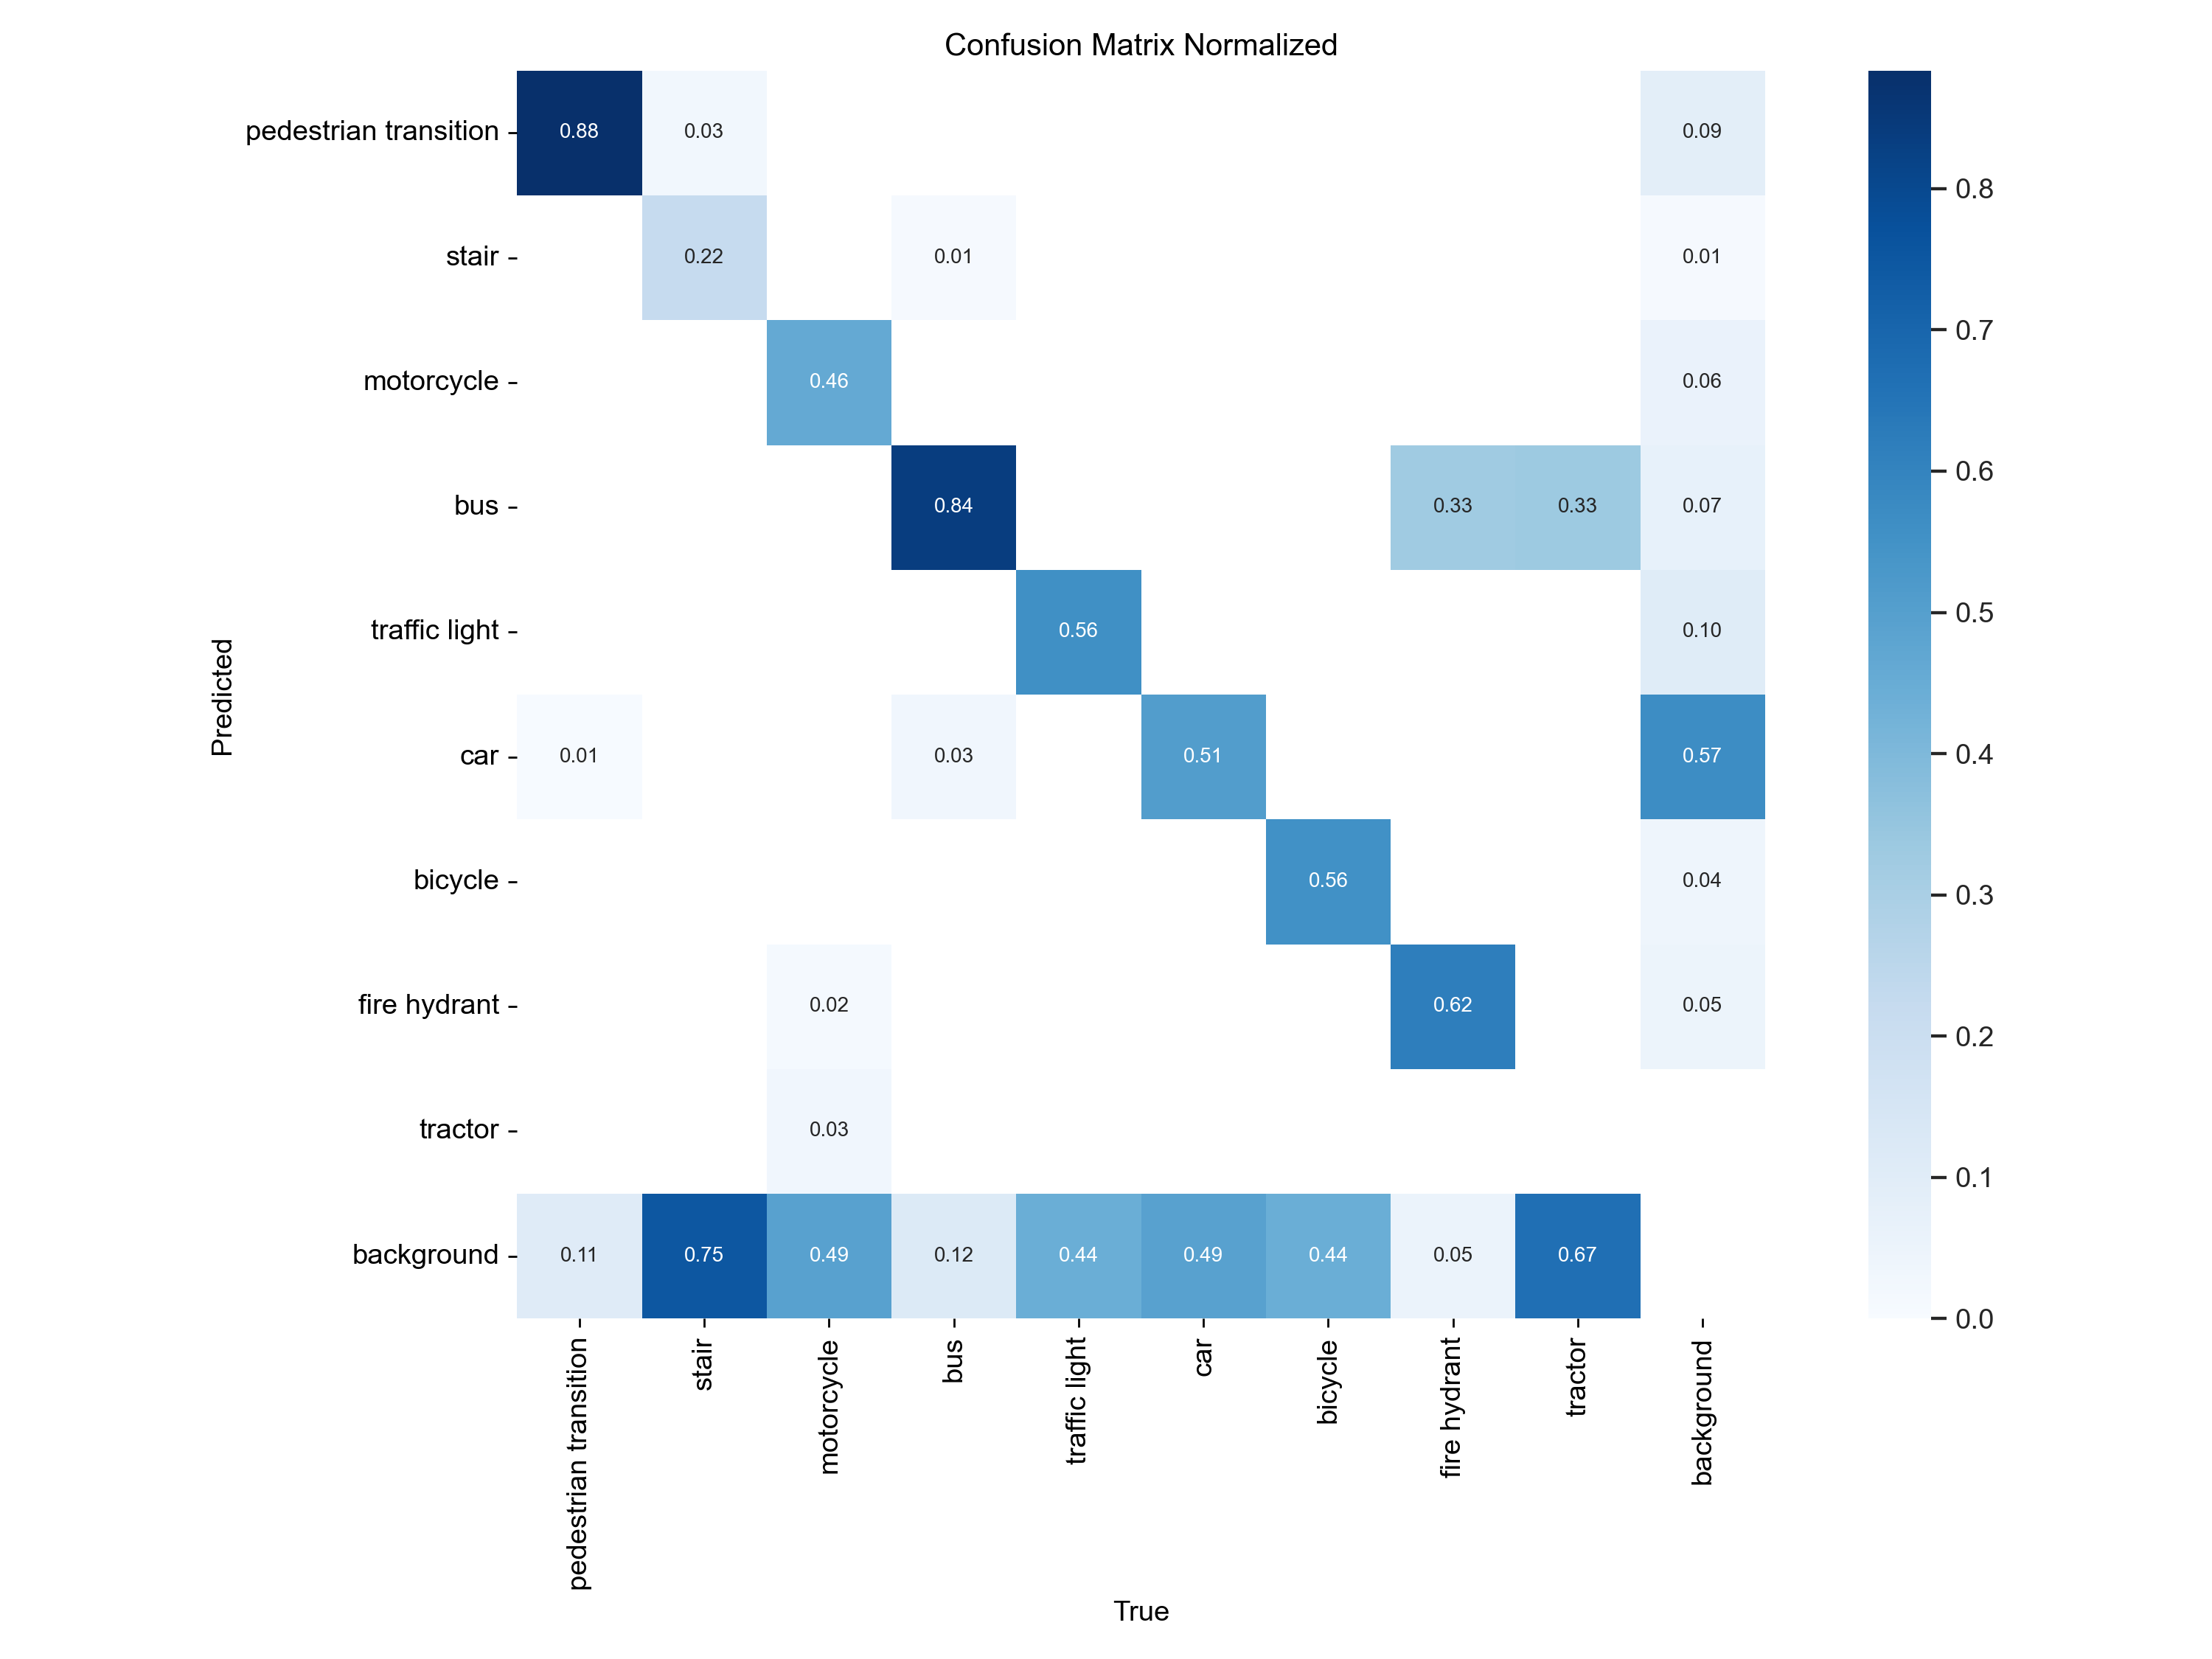
\includegraphics[width=0.9\linewidth]{
        imgs/imagecaptcha/confusion_matrix_normalized.png
    }
    \caption{Матрица ошибок для изображений валидационной выборки для модели 
    YOLOv8.}
    \label{fig:confusion}
\end{figure}
\vspace{-0.85cm}

После завершения обучения модель на основе YOLO была протестирована на реальных 
CAPTCHA, собранных с помощью автоматического парсера, реализованного на базе 
библиотеки Selenium. Тестирование проводилось в автоматическом режиме, имитируя 
реальные действия пользователя в браузере, что позволило оценить 
работоспособность системы в условиях, приближенных к реальной эксплуатации.

Сценарий тестирования предусматривал выполнение следующих шагов:

\begin{enumerate}
    \item автоматический переход к странице с CAPTCHA и активация чекбокса <<Я не 
    робот>>;
    \item извлечение изображения CAPTCHA (включая структуру сетки и текст 
    задания);
    \item определение целевого объекта из текста задания (например, «выберите все 
    изображения с автобусами»);
    \item разбиение изображения CAPTCHA на ячейки (в зависимости от размера сетки 
    -- 3×3 или 4×4);
    \item применение обученной модели для сегментации и классификации каждого 
    изображения или фрагмента;
    \item определение ячеек, содержащих нужный класс, и программная симуляция 
    кликов по ним;
    \item повторная попытка прохождения CAPTCHA в случае, если результат оказался 
    некорректным (что также фиксировалось в логах).
\end{enumerate}

Тестирование было организовано в виде цикла, позволяющего автоматически проходить 
CAPTCHA до тех пор, пока не будет достигнут положительный результат. Это 
позволило зафиксировать частоту ошибок модели и определить случаи, в которых 
требуются дообучение или оптимизация.

Рабочий процесс тестирования и взаимодействия модели с CAPTCHA представлен на 
блок-схеме ниже. Программная реализация процесса автоматизированного прохождения 
графических CAPTCHA представлена в приложении 3 (листинг~\ref{code:solve-captcha}).

\begin{figure}[H]
    \centering
    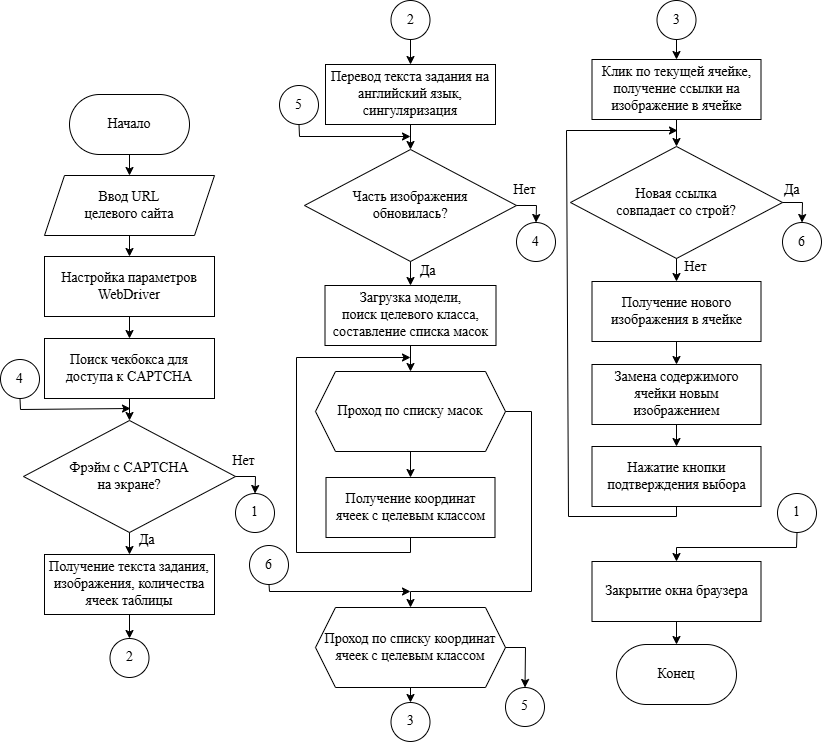
\includegraphics[width=1\textwidth]{imgs/imagecaptcha/solve_captcha_flow.png}
    \caption{Блок-схема процесса прохождения графических CAPTCHA.}
    \label{fig:solve-captcha}
\end{figure}
\vspace{-0.85cm}

Полученные данные используются для последующего анализа качества модели и 
корректировки процесса обучения. Основное внимание при анализе было уделено 
типам ошибок, сложности распознаваемых объектов и влиянию качества исходного 
изображения на точность сегментации.

\textbf{Тестирование системы автоматического распознавания речи для аудио CAPTCHA}

Для оценки эффективности реализованного решения по автоматическому распознаванию 
CAPTCHA в аудиоформате был проведён эксперимент, имитирующий поведение 
пользователя при взаимодействии с web-страницей, содержащей CAPTCHA-элемент. 
Процесс тестирования можно представить в виде последовательности этапов, 
автоматизированных с использованием средств управления браузером и сетевых 
запросов:

\begin{enumerate}
    \item инициализация среды тестирования: на данном этапе выполняется 
    конфигурация параметров браузера, включая отключение избыточной телеметрии, 
    блокировщиков всплывающих окон и иные настройки, необходимые для корректной 
    эмуляции пользовательского поведения;
    \item загрузка целевой web-страницы, содержащей CAPTCHA: осуществляется 
    открытие страницы, на которой встроен элемент reCAPTCHA с возможностью выбора 
    аудиоальтернативы;
    \item навигация к фрейму с элементом CAPTCHA и взаимодействие с ним: система 
    переходит к нужному вложенному фрейму и инициирует клик по чекбоксу 
    подтверждения <<Я не робот>>, что запускает механизм генерации задачи;
    \item определение типа CAPTCHA: если система предоставляет графическую 
    задачу, производится переход к интерфейсу, предлагающему аудиоверсию;
    \item переход к аудиоинтерфейсу: осуществляется переключение к 
    соответствующему фрейму и поиск HTML-элемента, содержащего ссылку на звуковой 
    файл CAPTCHA;
    \item инициализация получения аудиофайла: по извлечённой ссылке формируется 
    сетевой запрос для загрузки аудиофайла, как правило, в формате MP3, 
    полученный файл сохраняется в локальное хранилище для последующей обработки;
    \item обработка аудиофайла: аудиозапись проходит предварительную обработку, 
    включая преобразование формата в пригодный для распознавания (например, в 
    WAV), а затем передаётся в подсистему распознавания речи, основанную на 
    использовании облачного API;
    \item получение результата распознавания и его валидация: результат, 
    представленный в текстовой форме, сохраняется и автоматически вставляется в 
    соответствующее текстовое поле CAPTCHA на web-странице;
    \item завершение взаимодействия: выполняется отправка формы с введённым 
    ответом для проверки корректности распознанного текста.
\end{enumerate}

Блок-схема, иллюстрирующая приведенный алгоритм представлена на рис.~
\ref{fig:audio-solver}. Программная реализация алгоритма приведена в приложении 1 
(листинг~\ref{code:audiocaptcha-solve}).

\begin{figure}[H]
    \centering
    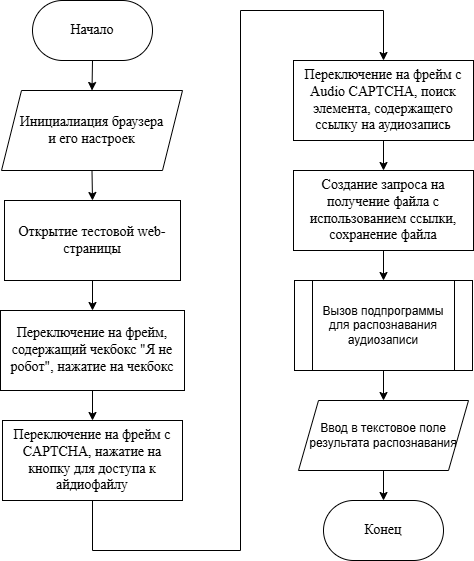
\includegraphics[width=0.55\linewidth]{imgs/audiocaptcha/captcha_solve.png}
    \caption{Блок-схема процесса прохождения Audio CAPTCHA.}
    \label{fig:audio-solver}
\end{figure}
\vspace{-0.85cm}

На всех этапах тестирования осуществлялся контроль корректности выполнения 
операций и логирование возникающих ошибок. Результаты распознавания оценивались 
на предмет соответствия требованиям CAPTCHA-системы. Отдельное внимание уделялось 
устойчивости решения к вариативности качества аудиофайлов и скорости отклика 
серверов, формирующих CAPTCHA.

Подобный подход к тестированию позволяет объективно оценить точность, надёжность 
и практическую применимость предложенного решения в условиях реального 
взаимодействия с web-средами.
